\documentclass[tikz,border=6pt]{standalone}
\usetikzlibrary{arrows.meta}

\begin{document}
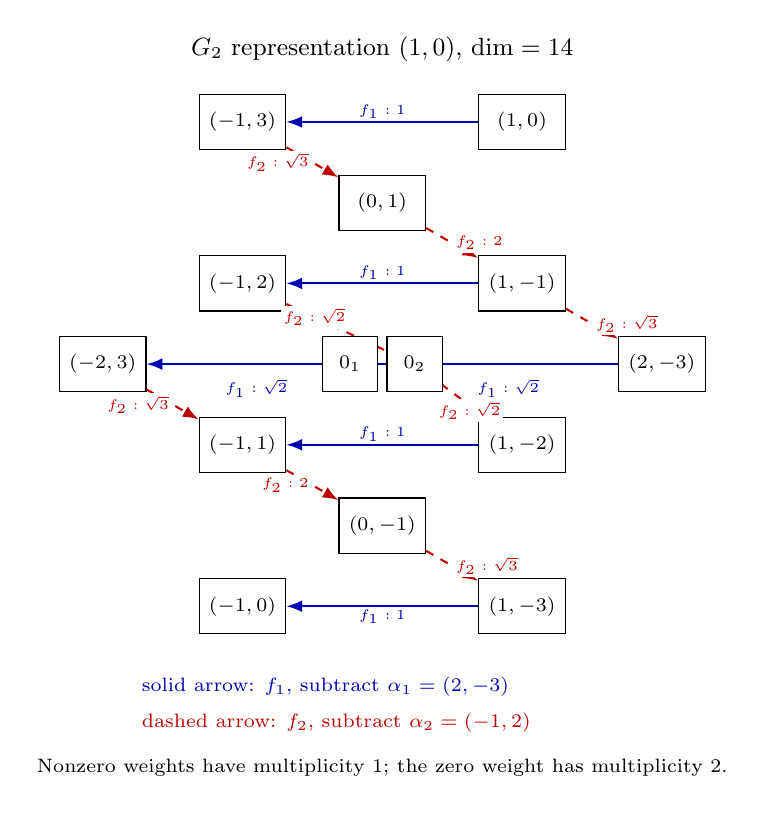
\begin{tikzpicture}[
  x=2.05cm,
  y=2.05cm,
  weight/.style={draw=black, fill=white, minimum width=11mm, minimum height=7mm, inner sep=1pt, font=\scriptsize},
  zerobox/.style={draw=black, fill=white, minimum width=7mm, minimum height=7mm, inner sep=1pt, font=\scriptsize},
  coef/.style={fill=white, inner sep=1pt, font=\tiny},
  edgeone/.style={blue!70!black, line width=0.75pt, -{Latex[length=2mm]}},
  edgetwo/.style={red!75!black, dashed, line width=0.75pt, -{Latex[length=2mm]}}
]
\node[font=\small] at (0,1.95) {$G_2$ representation $(1,0)$, $\dim=14$};

\node[weight] (p1z) at (0.866,1.5) {$(1,0)$};
\node[weight] (m1p3) at (-0.866,1.5) {$(-1,3)$};
\node[weight] (m2p3) at (-1.732,0) {$(-2,3)$};
\node[weight] (m1z) at (-0.866,-1.5) {$(-1,0)$};
\node[weight] (p1m3) at (0.866,-1.5) {$(1,-3)$};
\node[weight] (p2m3) at (1.732,0) {$(2,-3)$};

\node[weight] (p01) at (0,1) {$(0,1)$};
\node[weight] (p1m1) at (0.866,0.5) {$(1,-1)$};
\node[weight] (p1m2) at (0.866,-0.5) {$(1,-2)$};
\node[weight] (p0m1) at (0,-1) {$(0,-1)$};
\node[weight] (m1p1) at (-0.866,-0.5) {$(-1,1)$};
\node[weight] (m1p2) at (-0.866,0.5) {$(-1,2)$};

\coordinate (z1c) at (-0.20,0);
\coordinate (z2c) at (0.20,0);

\draw[edgeone] (p2m3) -- (z1c);
\draw[edgeone] (z1c) -- (m2p3);
\draw[edgeone] (p1m3) -- node[coef, below] {$f_1:1$} (m1z);
\draw[edgeone] (p1m2) -- node[coef, above] {$f_1:1$} (m1p1);
\draw[edgeone] (p1m1) -- node[coef, above] {$f_1:1$} (m1p2);
\draw[edgeone] (p1z) -- node[coef, above] {$f_1:1$} (m1p3);

\draw[edgetwo] (m2p3) -- node[coef, left] {$f_2:\sqrt{3}$} (m1p1);
\draw[edgetwo] (m1p1) -- node[coef, left] {$f_2:2$} (p0m1);
\draw[edgetwo] (m1p2) -- (z2c);
\draw[edgetwo] (m1p3) -- node[coef, left] {$f_2:\sqrt{3}$} (p01);
\draw[edgetwo] (p0m1) -- node[coef, right] {$f_2:\sqrt{3}$} (p1m3);
\draw[edgetwo] (z2c) -- (p1m2);
\draw[edgetwo] (p01) -- node[coef, right] {$f_2:2$} (p1m1);
\draw[edgetwo] (p1m1) -- node[coef, right] {$f_2:\sqrt{3}$} (p2m3);

\node[zerobox] (z1) at (z1c) {$0_1$};
\node[zerobox] (z2) at (z2c) {$0_2$};
\node[coef, text=blue!70!black] at (0.78,-0.15) {$f_1:\sqrt{2}$};
\node[coef, text=blue!70!black] at (-0.78,-0.15) {$f_1:\sqrt{2}$};
\node[coef, text=red!75!black] at (-0.42,0.29) {$f_2:\sqrt{2}$};
\node[coef, text=red!75!black] at (0.54,-0.29) {$f_2:\sqrt{2}$};

\node[font=\scriptsize, blue!70!black, anchor=west] at (-1.55,-2.0) {solid arrow: $f_1$, subtract $\alpha_1=(2,-3)$};
\node[font=\scriptsize, red!75!black, anchor=west] at (-1.55,-2.22) {dashed arrow: $f_2$, subtract $\alpha_2=(-1,2)$};
\node[font=\scriptsize] at (0,-2.5) {Nonzero weights have multiplicity $1$; the zero weight has multiplicity $2$.};
\end{tikzpicture}
\end{document}
